\subsection{Solution}\label{sec:solution}

The solution to the differential equation \eqref{eq:susyConditionTheta} is:
\begin{equation}\label{eq:susyConditionSolution}
\boxed{\sin\theta(c) = L \sqrt{c^2-1}; \quad 1 < c \leq \sqrt{1+L^{-2}}},
\end{equation}
where $L$ is an integration constant. As we will show below, it is the asymptotic separation of the D7-brane from the stack of the D3-branes, in the units of the spherical radius\footnote{The spherical part of our metric \eqref{eq:PWmetric} is multiplied by $R^2$.} $R$, namely $L$ above is really $ L/R$.
We have set $R=1$ so far. The upper bound of $c$ is set by the maximum of the sine.


Near the boundary, $c \approx 1 + z^2/2$, the solution behaves as
\begin{equation} \label{eq:thetaExpanded}
 \theta(z) \approx L \, z + \left(\frac{L}{8} +\frac{L^3}{6} \right) \, z^3 + O(z^5).
\end{equation} 
Moreover, keeping only the leading order of the large $L$ expansion, our solution reduces to the one found in the $AdS_5 \times S^5$ background, see \cite{Karch:2002sh} and \cite{Karch:2005ms}, i.e.
\begin{equation}
 \sin\theta(z)_\text{AdS} = L z,
\end{equation}
with the asymptotic expansion
\begin{equation}
\theta(z)_\text{AdS} \approx L z + \frac{L^3}{6} z^3 + O(z^5).
\end{equation}
The $L\gg 1$ limit ensures the upper bound for $c$ in \eqref{eq:susyConditionSolution} to reduce to the one from the AdS solution, namely $z_\text{max}=1/L$. 


As \cite{Karch:2005ms} explains, in the flat embedding space limit, this embedding describes a planar D-brane located at a constant distance $L$ away from the stack of $N$ D3-branes:
\begin{equation}
 L = \lim_{z \rightarrow 0 } \frac{R}{z} \sin\theta(z) = R \, L/R,
\end{equation}
where we explicitly stated $R$. Furthermore, this separation is proportional to the quark mass $m$:
\begin{equation}
 L = 2 \pi l_s^2 m.
\end{equation}


Figures in \ref{fig:vielbeins} show the vielbeins of the induced metric at the solution, from which we learn how the geometry of the embedding looks like at different values of $c$. First, observe the divergence at the horizon $c_\text{max}=\sqrt{1+L^{-2}}$. This is the location of the well-known enhançon locus, at $\theta = \pi/2$, see \cite{Buchel:2000cn} and \cite{Evans:2000ct}. The spheroid is undeformed at the boundary $c=1$, and becomes squashed until it vanishes at the enhançon. 

\begin{figure}[t!]
\begin{center}
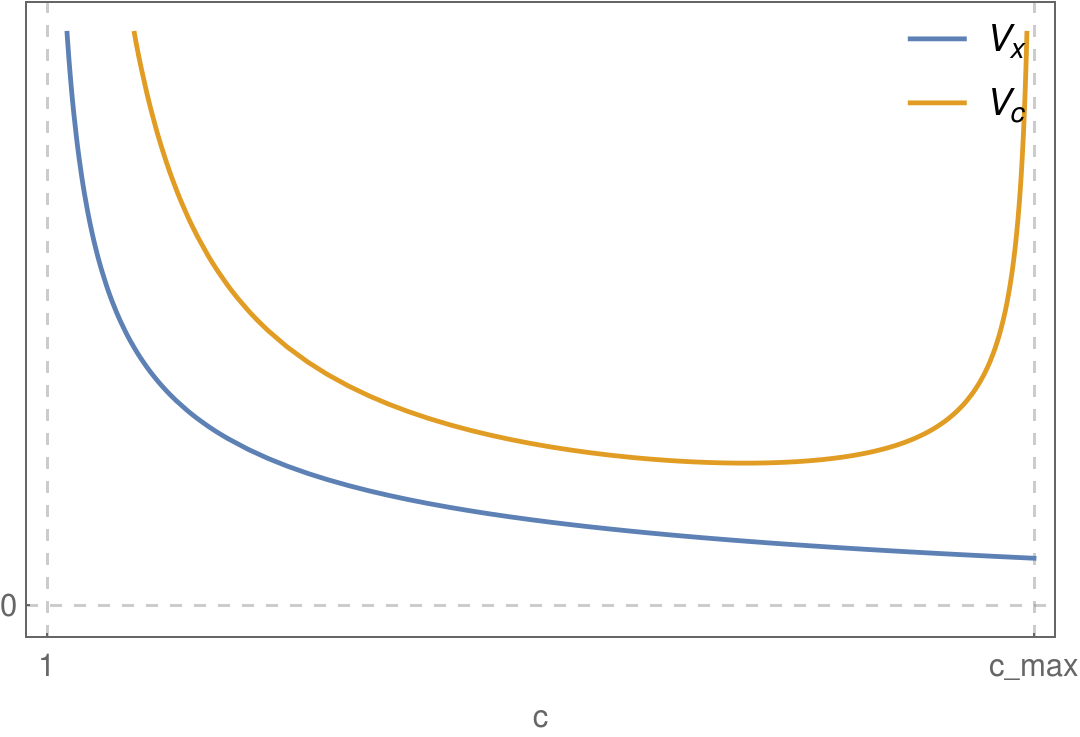
\includegraphics[width=0.6\textwidth]{pictures/vxvcb.png}
\end{center}
\vspace{0.05mm}
\begin{center}
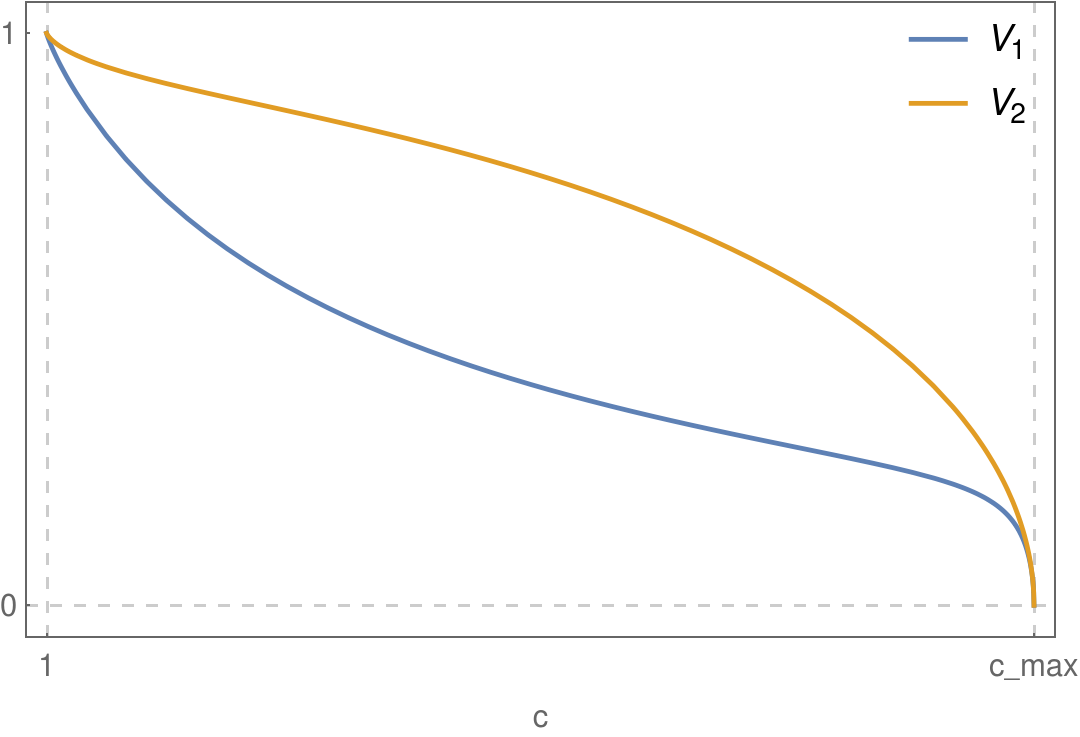
\includegraphics[width=0.6\textwidth]{pictures/v1v2b.png}
\end{center}
\caption{\label{fig:vielbeins} The vielbeins of the induced metric for the allowed values of $c$.}
\end{figure}
